\documentclass[10pt,a4paper]{paper}
\usepackage[utf8]{inputenc}
\usepackage{graphicx}
\usepackage{subcaption}
\usepackage{enumitem}
\usepackage{tikz}
\usetikzlibrary{calc}
\usepackage{pgfgantt}
\definecolor{TableOrange}{RGB}{255,151,46}
\definecolor{TableBlue}{RGB}{38,125,184}

\newcommand{\tup}[1]{{\langle #1 \rangle}}

\pdfoptionpdfminorversion=5


\title{Artificial Intelligence for the Automated Synthesis and Validation of Programs}
\begin{document}
\maketitle

\begin{abstract}
  Programming is nowadays a manual handcraft task however, the need to automate programming tasks increases every day: Programming errors, commonly known as {\em bugs}, cause undesired software behavior making programs crash or enabling malicious users to access private data. Just for 2017, the cumulative cost of software bugs is worldwide estimated in more than one trillion US dollars. 

  This research project investigates a novel approach for software development, that leverages {\em Artificial Intelligence} (AI), to increase the automation of the programming process and hence, reduce the chances of introducing software bugs. The project proposes to address {\bf program synthesis and program validation starting from {\em input-output} tests cases, and using {\em AI planning} as a problem solving engine}.

  Our work on this particular research topic is the recipient of the {\em 2016 distinguished paper award} at {\sc IJCAI} (the main international conference on AI) and has recently been accepted for publication at the {\em Artificial Intelligence Journal}, the premier international journal for research in AI. 

\end{abstract}
{\footnotesize {\bf Keywords:} Computer Science, Artificial Intelligence, Program Synthesis, Program Validation, AI planning.}



\section{Introduction}
\label{sec:introduction}

{\underline{Program Synthesis}} is the task of computing a program that satisfies a given formal specification of semantic correctness.

The 2008 PhD Thesis work by Armando Solar-Lezama, at the University of California Berkeley, showed that it is possible to encode program synthesis as a {\em Boolean logic SAT} problem and therefore, use {\em satisfiability modulo theories}~\cite{barrett:SMT:2009} to automatically compute programs~\cite{lezama2008program}. Since then, there has been a surge of practical interest in the idea of program synthesis in the formal verification community and related fields.

To illustrate this interest, in 2013 the unified framework {\sc SyGuS} for program synthesis problems was proposed~\cite{alur2013syntax}. Since then, there is a yearly competition ({\tt http://www.sygus.org}) comparing different approaches for program synthesis. Further since 2012, the {\sc US National Science Foundation} is funding the ExCAPE research project\footnote{\tt https://www.nsf.gov/awardsearch/showAward?AWD\textunderscore ID=1138996}, to transform the way programmers develop software by advancing the theory and practice of software synthesis (the ExCAPE research project is funded with a total amount of $\$3,750,000$). Last but not last, program synthesis have already been deployed in the real world and is part of the {\sc Flash Fill} feature of {\sc Microsoft Excel} that generates programs for string transformation~\cite{gulwani2011automating}.

Algorithmic approaches to program synthesis range over a wide spectrum, from {\em deductive synthesis} to {\em inductive synthesis}. In deductive program synthesis, a program is synthesized by constructively proving a theorem, employing logical inference and constraint solving~\cite{manna1986deductive}. On the other hand, inductive synthesis seeks to find a program matching a set of input-output examples~\cite{summers1977methodology,shapiro1983algorithmic}. It is thus an instance of learning from examples, also termed as {\em inductive inference} or {\em Machine Learning} (ML). Many current approaches to synthesis blend induction and deduction~\cite{seshia2015combining}; syntax guidance is usually a key ingredient in these approaches. Inductive synthesizers generalize from examples by searching a restricted space of programs. In ML, this space is called the {\em concept class}, and each element of that space is often called a {\em candidate concept}. The {\em concept class} is usually specified syntactically. Inductive learning is thus a natural fit for the syntax-guided synthesis problem introduced in this paper: the concept class is simply the set of permissible expressions.

Closely related to the aims of the project is the synthesis of {\it Finite State Controllers} (FSCs)~\cite{geffner:policies:IJCAI15}. The state-of-the-art algorithms for computing FSCs follow a {\it top-down} approach that interleaves {\it programming} the FSC with validating it~\cite{sergio:aprograming:ijcai16,segovia:FSC:JAIR2018}. To keep the computation of FSCs tractable, the space of possible solutions is bound by the maximum size of the FSCs. The computation of FSCs includes works that compile this task into another forms of problem solving so they benefit from the last advances on off-the-shelf solvers (e.g. {\em classical planning}~\cite{sergio:aprograming:icaps16}, {\em conformant planning}~\cite{Geffner:FSM:AAAI10}, {\em CSP}~\cite{Infantes:FSC:ECAI2010} or a {\em Prolog program}~\cite{Giacomo:FSM:ICAPS13}). The synthesis of programs from examples is also addressed in the classic AI field of {\em Inductive Logic Programming} (ILP)~\cite{muggleton1991inductive,Raedt:relationalML:book2008}. ILP arises from the intersection of {\em Machine Learning} and {\em Logic Programming} and deals with the development of inductive techniques to learn logic programs from  examples and background knowledge, that are expressed as logic facts.

{\underline{\em Program Validation}} is the task of proving, or disproving, the correctness of a given program with respect to a certain formal specification of its aimed semantics. Program validation is considered a necessary step for program synthesis. {\em Model checking} is the mainstream AI approach for the formal validation of programs and controllers~\cite{clarke1999model}. Current approaches for model checking reduces to graph search but, instead of enumerating reachable states one at a time, the state space is traversed considering large numbers of states at a single step. For instance, representing set of states and transition relations as logical formulas or binary decision diagrams, like in {\em symbolic model-checking} ~\cite{mcmillan1993symbolic}.



\section{Methodology}
\label{sec:methodology}
This research project will {\bf investigate the integration of {\em AI planning} into the {\em Test Driven Development} paradigm for the automatic synthesis and validation of programs}. Here we briefly introduce this technology:
\begin{itemize}
\item {\bf AI Planning (AIP)} is the Artificial Intelligence component that studies the synthesis of sets of actions to achieve some given objectives~\cite{ghallab2004automated}. AIP arose in the late ’50s from converging studies into {\em combinatorial search}, {\em theorem proving} and {\em control theory} and now, is a well formalized paradigm for problem solving with algorithms that scale-up reasonably well. State-of-the-art planners are able to synthesize plans with hundreds of actions in seconds time~\cite{geffner2013concise}.  The mainstream approach for AIP is {\em heuristic search} with heuristics derived automatically from the problem representation~\cite{mcdermott1996heuristic,bonet2001planning}.  Current planners add other ideas to this like {\it novelty exploration}~\cite{geffner:psimulators:IJCAI17}, {\it helpful actions}~\cite{hoffmann2001ff}, {\it landmarks}~\cite{helmert2006fast}, and {\it multiqueue best-first search}~\cite{richter2010lama} for combining different heuristics.
  
\item {\bf Test driven development (TDD)}~\cite{beck:TDD:2003} is a popular paradigm for software development that is frequently used in {\it agile methodologies}~\cite{cohen2003agile}. In TDD, test cases are created before the program code is written and they are run against the code during the development, e.g. after a code change via an automated process. When all tests pass, the program code is considered {\em complete} while when a test fails, it pinpoints a {\em bug} that must be fixed from the program code. Tests cases are a natural form of program specification, programmers often claim {\em 'code that is difficult to test is poorly written'}. Further, tests alert programmers of bugs before handing the code off to clients (the cost of finding a bug when the code is first written is considerably lower than the cost of detecting and fixing it later). %Last but not least, writing a thorough set of tests cases forces programmers to think through inputs, outputs, and error conditions of programs. 
\end{itemize}

\subsection{Synthesis and validation of programs as AI planning}
Our current research already shows that AI planners can synthesize programs for non trivial tasks like sorting lists, traversing graphs or manipulating strings~\cite{jimenez2015computing,sergio:aprograming:icaps16,sergio:aprogramingb:ijcai16,sergio:aprograming:ijcai16,segovia2017generating,segovia:FSC:JAIR2018,segovia:programs:AIJ19}. Table~\ref{tab:programs} reports the time invested by the AI planner {\sc FD}~\cite{helmert2006fast} to solve the following programming tasks: computing the $n^{th}$ term of the {\em summatory} and  {\em Fibonacci} series, {\em reversing} a list, {\em finding} an element (and the {\em minimum} element) in a list, {\em sorting} a list and traversing a binary tree, or building a {\em parser} for simple arithmetic operations. 
 
\begin{table*}[hbt!]
  \centering
\begin{small}  
\begin{tabular}{l@{\hspace*{30pt}}r@{\hspace*{5pt}}}
 \textbf{Programming Task} & \textbf{Time (seconds)} \\\hline
Summatory		&	1\\
Fibonacci		&	5\\
Reverse			&	22\\
Find                    &       336 \\
Minimum                 &       284 \\
Sorting			&	30\\
Tree  		        &	165\\
Parser                  &       45
\end{tabular}
\end{small}  
\caption{\small Time to synthesize the programs with the AI planner {\sc FD}~\cite{helmert2006fast} on a processor {\em Intel Core i5 3.10GHz x 4} and with a 4GB memory bound.}
\label{tab:programs}
\end{table*}

We now give more details of our method for program synthesis and validation. Given a {\em TDD programming} task, our approach is modeling and solving it as it were an {\em AI planning} task. Briefly the {\bf state variables} of this AIP task are {\em fluents} of the kind:
\begin{itemize}
\item {\tt var:=value}, that encode the value of the program variables.
\item {\tt program(line):=instruction}, that encode the instructions at the different program lines.
\item {\tt pcounter:=line}, encoding which is the current program line.
\end {itemize}

The {\bf initial/goal states} of the AIP task encode the initial/final values of the program variables and are given by the input/output tests of the TDD programming task.

Finally, program instructions are encoded using two kinds of AIP {\bf actions}:
\begin{itemize}
\item {\it Programming actions}, that assign an instruction in the {\em instruction set} to a given program line.
\item {\it Execution actions}, execute the instruction assigned to the current program line.
\end{itemize}
We implement this encoding using standard planning languages, such as PDDL~\cite{fox2003pddl2}, so the AIP tasks resulting from our encoding can be solved with off-the-shelf planners, like the {\sc FD} planning system~\cite{helmert2006fast}. The programs synthesized with this approach are guaranteed to be bug-free over given sets of {\em input-output} tests cases.

Interestingly, our PDDL encoding allows also program validation by (1), specifying the lines of the program to validate (i.e. the {\tt program(line):=instruction} fluents) in the initial state of the AIP task and (2), disabling the mentioned {\it programming actions} so only {\it execution actions} are applicable.


\subsection{Evaluation}
\label{sec:evaluation}

The performance of our approach for the synthesis and validation of TDD programming tasks will be evaluated with regard to (1 )the {\bf computation time} and (2), the {\bf memory} invested in the synthesize and the validation of the aimed programs.

We will evaluate our approach in programming tasks of two different kinds:
\begin{itemize}
\item {\em Real-world benchmarks}: The GRPS group is currently leading the four-year research project TIN2017-88476-C2-1-R from the {\em Spanish national plan} in which {\em AI Planning} and {\em activity recognition} is applied to different real-world domains such as {\em domotics}, {\em tourism}, {\em traffic control} and {\em robotics}. Interestingly many activities in these domains can be understood as simple programs. For instance, Figure~\ref{fig:activity} shows a four-line program (pictured as a finite state machine) that represents the sequence of instructions required for the {\em making a buttered toast} activity. We plan to evaluate our approach in synthesis and validation tasks coming from these real-world domains. 

\begin{figure}[hbt!]
\begin{center}
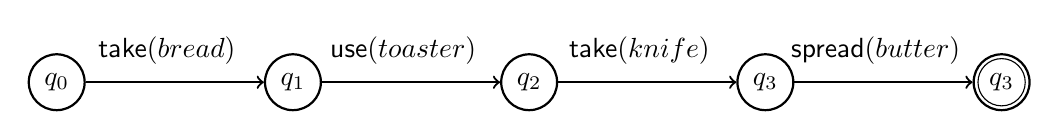
\begin{tikzpicture}
\node [thick,draw,circle] at (1,1.1) (x) {$q_0$};
\node [thick,draw,circle] at (4,1.1) (y) {$q_1$};
\node [thick,draw,circle] at (7,1.1) (v) {$q_2$};
\node [thick,draw,circle] at (10,1.1) (w) {$q_3$};
\node [thick,draw,circle] at (13,1.1) (z) {$q_3$};
\draw (13,1.1) circle (.3cm);

\draw [thick,->] (x) to (y);
\draw [thick,->] (y) to (v);
\draw [thick,->] (v) to (w);
\draw [thick,->] (w) to (z);

\node at (2.4,1.5) {$\mathsf{take}(bread)$};
\node at (5.4,1.5) {$\mathsf{use}(toaster)$};
\node at (8.4,1.5) {$\mathsf{take}(knife)$};
\node at (11.4,1.5) {$\mathsf{spread}(butter)$};

\end{tikzpicture}
\end{center}
\caption{\small Four-line program representing the activity of {\em making a buttered toast}.}
\label{fig:activity}
\end{figure}


\item {\em Theoretical benchmarks}: Classic programming tasks are a neat touchstone to assess the performance of our approach. For instance, programs for the computation of mathematical/logic series, string manipulation and for the management of data structures such as {\em lists}, {\em queues}, {\em stacks} or {\em trees}. Figure~\ref{fig:list} shows a synthesized program for traversing a linked list. The program is pictured as a {\em finite state machine}: The machine nodes mount to the different program lines while edges are tagged with a {\em condition/instruction} label, that denotes the condition (over the program variables) under which program instructions are taken.  
\end{itemize}


\begin{figure}[hbt!]
\begin{center}
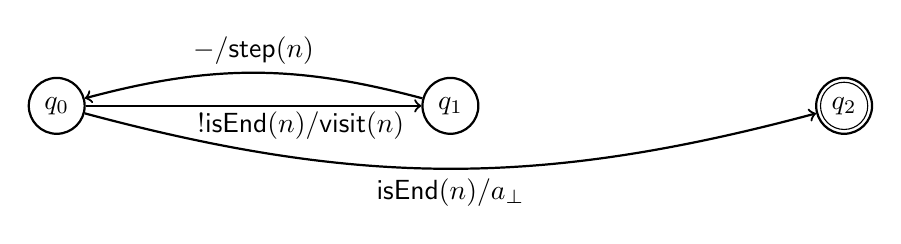
\begin{tikzpicture}
\node [thick,draw,circle] at (1,1.1) (x) {$q_0$};

\node [thick,draw,circle] at (6,1.1) (y) {$q_1$};

\node [thick,draw,circle] at (11,1.1) (z) {$q_2$};

\draw (11,1.1) circle (.3cm);

\draw [thick,->] (x) -- (y);

\draw [thick,out=345,in=195,->] (x) to (z);

\draw [thick,out=165,in=15,->] (y) to (x);

\node at (4.1,0.85) {$!\mathsf{isEnd}(n)/\mathsf{visit}(n)$};
\node at (3.5,1.8) {$-/\mathsf{step}(n)$};
\node at (6,0) {$\mathsf{isEnd}(n)/a_\bot$};
\end{tikzpicture}
\end{center}
\caption{\small Synthesized program to solve the programming task of traversing a linked list ($n$ is a variable that points to a node of the linked list).}
\label{fig:list}
\end{figure}



\subsection{Specific Objectives}
\label{sec:objectivos}

The programs objects of study in this project are characterized by these tree dimensions:
\begin{enumerate}
\item Number of {\em program lines}.
\item Number and domain of the observable {\em program variables}.
\item Size of the available {\em instruction set}.
\end{enumerate}  

For instance the program of Figure~\ref{fig:list}, for traversing linked lists, is generated using three program lines, one observable variable ($\mathsf{isEnd}(n)$ that has Boolean domain and indicates when $n$ points to the end of the given linked list), and an instruction set that comprises two instructions ($\mathsf{visit}(n)$, that marks the list node assigned to $n$ as {\em visited} and $\mathsf{step}(n)$, that advances $n$ to the next node in the linked list).


The specific objective of this project is to study the performance of our approach (in terms of computation time and memory) for the automated synthesis and validation of TDD programming tasks coming from the domains described in the previous subsection. In more detail, the two specific objectives of this project are:
\begin{enumerate}
\item To study the performance of our Artificial Intelligence approach for the {\bf synthesis of programs} up to: {\bf 10 program lines}, {\bf 10 observable variables} with binary domain and, an instruction set that comprises {\bf 10 instructions}. 
\item To study the performance of our Artificial Intelligence approach for the {\bf validation of programs} up to: {\bf 15 program lines}, {\bf 15 observable variables} with binary domain and, an instruction set that comprises {\bf 15 instructions}. 
\end{enumerate}

Despite setting bounds for the programs size and kind, challenging programming tasks can be addressed using {\em problem decomposition}. With this regard, our AIP encoding already supports callable procedures to decompose a given programming task into simpler modules and to enable recursive solutions~\cite{sergio:aprograming:icaps16,sergio:aprograming:ijcai16,segovia:FSC:JAIR2018,segovia:programs:AIJ19}.



\section{Workplan}
\label{sec:workplan}

We designed a 24-month workplan plan for the {\bf development of a user-interactive program synthesizer} that (1), takes as input a set of test cases that specify the TDD programming task to solve and (2), outputs a program source code that passes these tests with a bug-free guarantee.

In the particular case that the {\em program synthesizer} receives an additional input specifying the program source code, it outputs a validation certificate guaranteeing that the input program passes the given test cases. Figure~\ref{fig:gantt} details the proposed 24-month timeline for the project. A deliverable is provided at the end of each task.

\begin{figure}[hbt!]
\begin{ganttchart}[
  hgrid,
  group progress label node/.append style={below=3pt},
  canvas/.append style={label=below:} ]{1}{12} 
\ganttbar[bar/.append style={line width=1pt, draw=TableBlue,fill=TableBlue,fill opacity=0.6274509804}]{Design (6 months)}{1}{3} \\
\ganttbar[bar/.append style={line width=1pt, draw=TableBlue,fill=TableBlue,fill opacity=0.6274509804}]{Development (6 months)}{4}{6}\\
\ganttbar[bar/.append style={line width=1pt, draw=TableBlue,fill=TableBlue,fill opacity=0.6274509804}]{Experiments \& dissemination (12 months)}{7}{12}
\end{ganttchart}
\caption{\small Work-plan for developing a user-interactive program synthesizer/validator.}
\label{fig:gantt}
\end{figure}


\begin{enumerate}
\item {\bf T1. System design (months 1-6})
  \begin{small}
    \begin{enumerate}
    \item Design of the test-case specification. Programming tasks are specified as a set of {\em input-output} tests cases plus the available instruction set. 
    \item Experimental design. Experiments will comprise taking time and memory measurements to evaluate the resources required by our approach to solve the given TDD programming/validation tasks.
    \item Evaluation of the different AI planners available, with special attention to the planners that get the best results at the IPC-2018. 
      \end{enumerate}
  \end{small}

{\small{\bf\em  Deliverable T1:} Technical report with the specifications of the system design.}
  
  \item {\bf T2. Development of the system architecture (months 7-12})
    \begin{small}
      \begin{enumerate}
      \item The programming-into-planning compiler ({\em Compiler 1}). This system component parses the {\em TDD programming task} and produces an {\em AIP task} encoded in the standard planning language PDDL.
      \item The plan-into-program compiler ({\em Compiler 2}). This system component extracts the program code and the corresponding validation certificate from the solution plan produced by an off-the-shelf AI planner.
      \end{enumerate}
\end{small}      

\begin{figure}[hbt!]
\tikzstyle{block} = [draw, draw=TableBlue,fill=TableBlue,fill opacity=0.6274509804, rectangle, minimum height=3em, minimum width=6em]
\tikzstyle{input} = [coordinate]
\tikzstyle{output} = [coordinate]
\begin{center}
\begin{tikzpicture}[auto, node distance=2cm,>=latex']
    % We start by placing the blocks
    \node [input, name=input] {};
    \node [block, right of=input, node distance=4cm] (compiler1) {Compiler 1};
    \node [block, below of=compiler1, node distance=2cm] (planner) {AI Planner};    
    \node [block, below of=planner, node distance=2cm] (compiler2) {Compiler 2};
    \node [output, right of=compiler2, node distance=3cm] (output) {Program};


    % Once the nodes are placed, connecting them is easy. 
    \draw [->] (input) -- node {Programming task} (compiler1);
    \draw [->] (compiler1) -- node[] {AIP task} (planner);
    \draw [->] (planner) -- node[] {Solution plan} (compiler2);        
    \draw [->] (compiler2) -- node[] {Program}(output);
\end{tikzpicture}
\end{center}  
\caption{\small System architecture for the synthesis and validation of TDD programs.}
\label{fig:architecture}
\end{figure}

{\small{\bf\em Deliverable T2:} Open repository with the source code of the system architecture and the corresponding benchmarks.}
    
\item {\bf T3. Experiments and dissemination of results (months 13-24}).
   \begin{small}
      \begin{enumerate}
      \item Reporting the experimental performance of our AIP approach for solving diverse TDD programming tasks. This task will follow an iterative workflow over the following subtasks:
      \begin{enumerate}
      \item Executing the system architecture in the {\em theoretical benchmarks} described in Section~\ref{sec:evaluation}.
      \item Analysis and validation of the obtained results.
      \item Tuning and repairing the system components, evaluation metrics and benchmarks according to the obtained results.                 
      \item Executing the system architecture in the {\em real-world benchmarks} introduced in Section~\ref{sec:evaluation}.
      \item Analysis and validation of the obtained results.         
      \item Tuning and repairing the system components, evaluation metrics and benchmarks according to the obtained results.                 
      \end{enumerate}
      \item Dissemination of the obtained theoretical and empirical results by submitting papers to top international conferences and journals in AI.        
      \end{enumerate}
\end{small}        
{\small{\bf\em  Deliverable T3:} Final report with the obtained conclusions and produced publications.}
\end{enumerate}

\subsection{Workload}

{\em Tasks ({\bf T1-T3})} will be developed by the three mentioned members of the research group: Sergio Jiménez, Eva Onaindia and Diego Aineto.

In addition, we plan to hire a master student for 6 months to assist in the completion of two tasks, {\bf T3(a,i)} and {\bf T3(a,iv)}. The detailed responsability of the student will be:
\begin{enumerate}
\item Executing the scripts of the system architecture.
\item Collecting the output data.
\item Presenting the output data in a easy-readable format.
\end{enumerate}


\subsection{Budget}
Here we show the detailed desctiption of the two-year budget for the development of the proyect.

\begin{table}[hbt!]
\begin{small}  
  \begin{tabular}{clc|l}
    {\bf Priority} & {\bf Description} & {\bf Term} & {\bf Euros} \\\hline
1 & {\scriptsize Difusión de las actividades del grupo} & 2018, 2019 & 2,000\\    
2 & {\scriptsize Viajes, manutención y alojamiento grupo de investigación} & 2018 & 1,500\\
3 & {\scriptsize Viajes, manutención y alojamiento grupo de investigación} & 2019 & 1,500\\
4 & {\scriptsize Viajes, manutención, alojamiento y ponencias investigadores invitados} & 2018 & 1,500\\
5 & {\scriptsize Viajes, manutención, alojamiento y ponencias investigadores invitados} & 2019 & 1,500\\\hline
\multicolumn{3}{l|}{} & 8,000 \\
  \end{tabular}
\end{small}
\caption{\small Two-year budget for the development of the proyect.}
\end{table}



\section{Disemination and exploitation of the research results.}
\label{subsec:beneficios}
AIP has recently shown successful in {\em program testing} to generate {\em attack plans} that completed non-trivial software security tests~\cite{hoffmann2015simulated,steinmetz2016revisiting,shmaryahu2016constructing,steinmetz2016goal}. Promising research opportunities come from the application of AIP to {\em program synthesis} given that, {\em program synthesis} with a tests base, can be seen as the {\em program testing} dual.

In fact, our current work on {\em program synthesis} with AIP already produced several {\bf publications at top international conferences and journals on Artificial Intelligence}~\cite{segovia2017generating,sergio:aprogramingb:ijcai16,sergio:aprograming:ijcai16,sergio:aprograming:icaps16,segovia:FSC:JAIR2018,segovia:programs:AIJ19} and is the recipient of the {\it 2016 distinguished paper award} at the International Joint Conference on Artificial Intelligence, the main international conference on {\em Artificial intelligence}. 

The main benefit of this project is to provide new insights into the current understanding of how AI can assist programmers in the software development. In more detail, the expected benefits for this particular research project are four-fold:
\begin{enumerate}
\item A new {\bf evaluation methodology for the {\em Synthesis and Validation of Programs}}. The application of the exiting AIP technology to program synthesis can provide new evaluation metrics that assess how well a program covers a set of {\em input-output} test cases.  
\item An empirical {\bf study on the performance of the state-of-the-art AI planners for the {\em Synthesis and Validation of Programs}}. Research in AI algorithms is too often tested with laboratory problems and AIP is not an exception. Most of the new planning algorithms are only tested within the benchmarks of the International Planing Competition~\cite{vallati:IPC:AI15}. This project will help to meet the computational and expressiveness limits of AI planners when addressing real-world programming tasks. 
\item The {\bf development of open software and open benchmarks for the {\em Synthesis and Validation of Programs}}. We strongly belief that reproducibility and open knowledge are essential to the advance of the research on computer science. With this regard, we plan to develop a {\em github} repository where we make available the developed source code and benchmarks.
\item {\bf International dissemination of the obtained scientific results}. The scientific results obtained during the development of the project will be submitted to top Artificial Intelligence conferences (such as IJCAI, AAAI, ICML and ICAPS) and to the main journals in the AI field (such as AIJ, JMLR and JAIR).
\end{enumerate}

\vspace{0.3cm}


\begin{scriptsize}
\bibliography{AI-programming}
\end{scriptsize}
\bibliographystyle{ieeetr}

\end{document}
